\chapter{Methodology}
\label{chapter:chapter03}

In the following chapter is explained the different parts of the problem to solve and 




\section{Problem Design}

The problem established is described as given a database of n users, an optimal arrangement of these users must be found, this arrangements puts each user in a group, with the users being in the same group that optimizes their predefined preference as described in [ref I], this optimization is described as finding the less distance between the level of experience of the users inside the same group, finding the less distance among an ontology of interests, where similar interests related interests are in the same branch, as well as the having a group size near the optimal group size which is defined as between 4 and 5, and the percentage of participation which is how much the users may participate in the group, maximizing in the most participation.

The solution is then the number of the group for each user, serving it as an id only, without any relevance in the order the groups are presented, only that the preference of the users is mantained within the group, this can more clearly be seen in ref[fig. ] and [fig. ]

\begin{figure}[dataset]
    \caption{This is an example of a dataset of 9 users, each with their id, exp, 3 different interests and a participation percentage}
    
\end{figure}
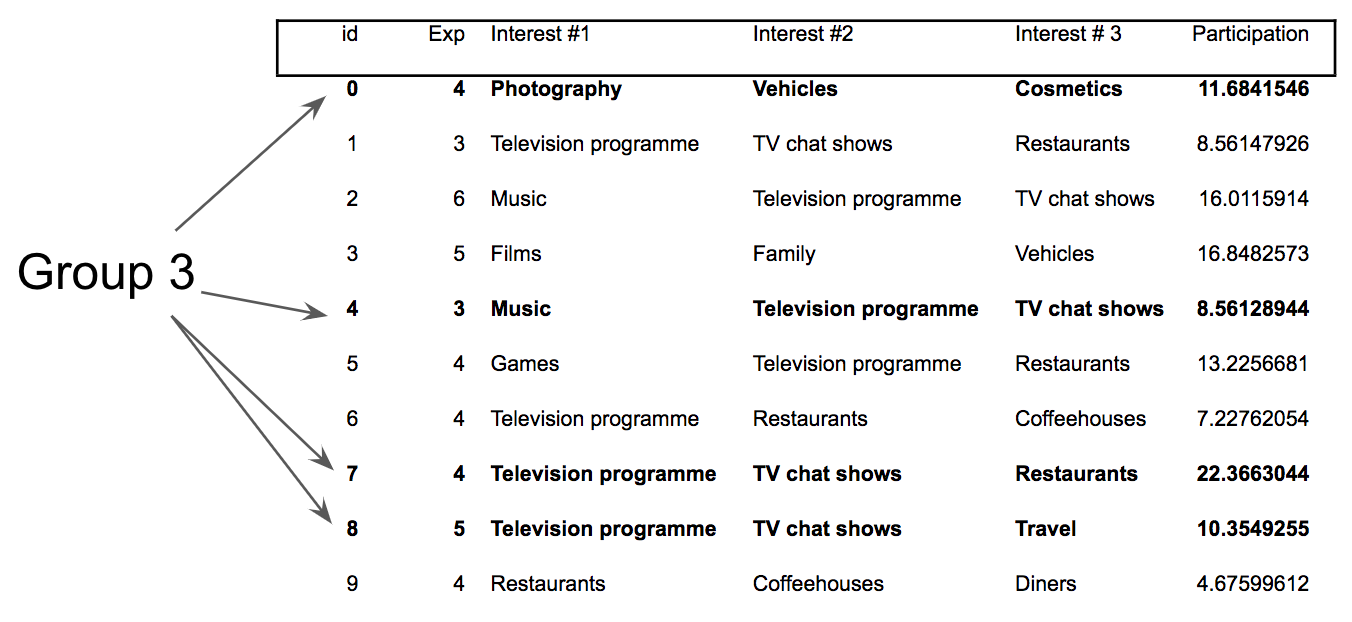
\includegraphics[]{images/dataset_eg.png}


\section{Objective Functions}

En la siguiente sección se describen distintas funciones objetivo para predecir la preferencia del usuario y la estabilidad del grupo, buscando minimizar el valor de cada una de ellas.

\subsection{Tamaño del Grupo}

Para propósitos de la investigación el tamaño ideal del grupo se considera como de \textbf{4 a 5} personas, ya que este tamaño usualmente permite una participación de todos los usuarios que pertenezcan al grupo. Es posible que puedan existir grupos de \textbf{3 o 6} personas, pero esto no es lo ideal, sin embargo se deja abierta la posibilidad en caso de que alguna otra característica como los intereses en común o el estilo de participación resulten más relevantes para el grupo que su tamaño.

La función para calcular este objetivo mide la cercanía al valor \textbf{4.5}, ya que 4 y 5 se consideran igual de ideales y 4.5 es simplemente el promedio entre ambos valores. Esta función esta definida a continuación:\ref{eq_group_size}

\begin{equation} \label{eq_group_size}
    f = | groupSize - 4.5|
\end{equation}

\subsection{Nivel de experiencia}

El nivel de experiencia en el lenguaje hace referencia al estándar CEFR\cite{}. Los valores que se consideran para ello son A1, A2, B1, B2, C1 y C2, por lo que se les asigna un valor numérico a cada uno siendo A1 0 y C2 5. Lo que se busca principalmente es que los usuarios dentro del grupo no tengan mucha variación en cuanto a su nivel de experiencia. De esta forma el vocabulario usado no se considera tan avanzado para integrantes con un nivel bajo ni tan sencillo para integrantes más avanzados. La fórmula\ref{eq_nivel} consiste en una desviación estándar del valor del nivel de cada uno de los integrantes, de forma ideal que sea alcanzado el 0 indicando que todos los usuarios del grupo forman parte del mismo.

\begin{equation} \label{eq_nivel}
    \sigma = \sqrt{\frac{1}{n-1} \sum_{i=1}^n (x_i - \overline{x})^2}
\end{equation}

\subsection{Intereses}

Para calcular la similitud entre intereses se usa una estrategia similar a Madylova y Gunduz \cite{taxonomy_semantic_similarity} donde los intereses son considerados como un vector valores en los que se señala una cantidad que indica el orden jerárquico de acuerdo a la ontología definida por la red social de Facebook, por ejemplo si un usuario tiene como intereses: Los perros, Correr y las Citas, su vector de intereses se estaría dado por los valores en la Figura \ref{fig:interests_table}. En la parte de arriba se indica el valor de la jerarquía, en la parte de abajo se normaliza usando \(1/(1+v)\), después se eligen los valores mayores de cada una de las columnas de esta forma da el vector resultante como se muestra en la Figura \ref{fig:interests_vector} \\

% Cambiar por tabla
\begin{figure}
    \centering
    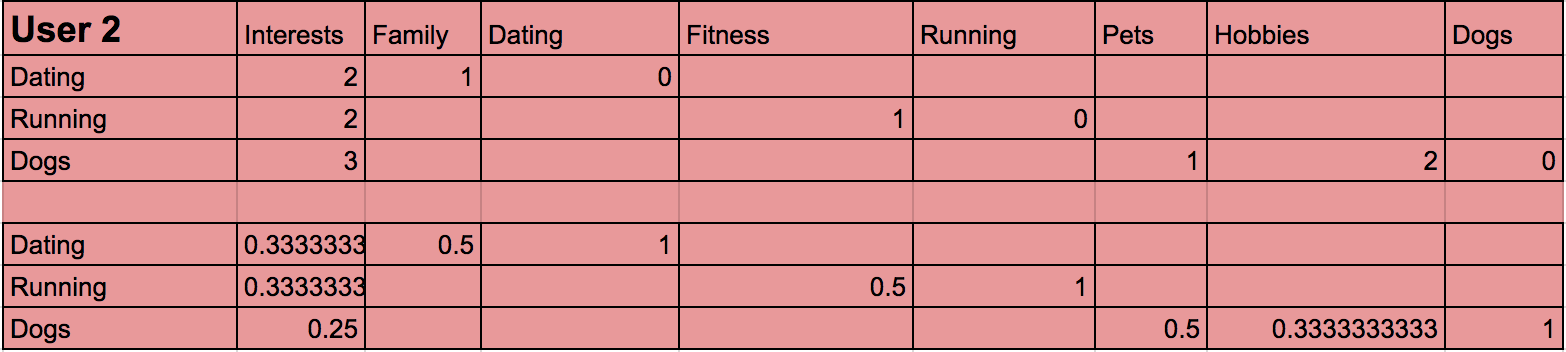
\includegraphics[width=150mm]{interests_table.png}
    \caption{Tabla de valores de Intereses}
    \label{fig:interests_table}
\end{figure}

% Cambiar por tabla
\begin{figure}
    \centering
    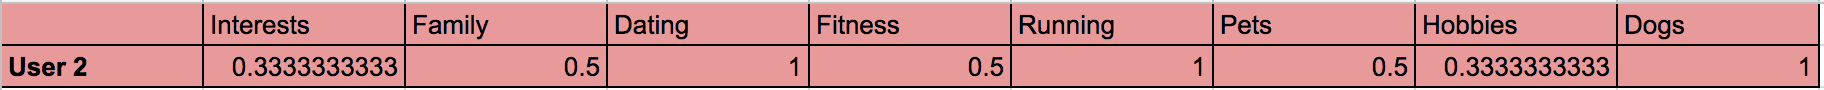
\includegraphics[width=150mm]{interests_vector.png}
    \caption{Vector de Intereses}
    \label{fig:interests_vector}
\end{figure}

Para calcular que tan similar es un usuario con respecto a otro se usa la formula de distancia cosenoidal, que se muestra en la ecuación \ref{eq_cos_sym} donde \(A\) es el vector de intereses del primer usuario y \(B\) es el vector de intereses del segundo. Cabe destacar que es muy frecuente que los vectores de intereses de los usuarios contengan ceros al momento de compararlos, de tal manera que si el resultado de la función da como resultado exactamente 0, significa que ambos usuarios no tienen nada en común. 

\begin{equation} \label{eq_cos_sym}
    \cos(\theta) = \frac{ \sum\limits_{i=1}^{n}{A_i  B_i} }{ \sqrt{\sum\limits_{i=1}^{n}{A_i^2}}  \sqrt{\sum\limits_{i=1}^{n}{B_i^2}} }   
\end{equation}
\begin{equation}\label{eq_interests}
	f = 1 - \cos(\theta) 
\end{equation}

\subsection{Estilo de Participación}

Para esta función trato de buscarse en la literatura algún tipo de función matemática ya definida para evaluar que tipo de roles son los que provocan que haya una participación más homogénea dentro del grupo dependiendo del rol funcional de cada uno de los participantes y su compatibilidad entre si. Sin embargo no se encontró ninguna, por lo que fue necesario definirla por medios propios. Afortunadamente se cuenta con una definición concreta de como debe ser la función, tomar en cuenta como parámetro los roles funcionales de cada usuario y dando como resultado de su evaluación el nivel de participación del grupo de forma numérica con la idea de optimizar dicho resultado.

Es por esto que al hacer el análisis de los datos como se describe en la sección de Experimentación [ref], se toman en cuenta 

%Ya que no hay ningún paper que diga que función usar para esto se le hizo un análisis de datos al AMI meeting corpus para ver que relación había entre el número de silencios y la homogeneidad de las participaciones de acuerdo con los funcional roles de Benne & Sheats, y pues resulta que si hay una correlación con respecto al porcentaje de participaciones por lo que se uso esta medida para tratar de predecir la interacción del grupo, considerando que esta participación debe ser homogénea entre ellos por lo que es el inverso a la suma de las participaciones y así...

% - Esta función está pensada para que pueda haber fluidez para hablar dentro del grupo; minimizando los silencios y aumentando volviendo el número de participaciones uniforme con respecto a los usuarios.
% - Hay mucha literatura mencionando porque esto funciona, pero nadie dice una medida matemática que se pueda usar para esto...
% - Se hizo un análisis de los datos a la base de datos de AMI, y se descubrió que los silencios y las participaciones están directamente relacionados con respecto a una medida de participación dentro del grupo, en efecto, se necesita.
% - TODOS los usuarios se comportan como protagonistas en algún punto, ya que este es el estilo que nos interesa optimizar es en el que nos basamos.
% - Más adelante al momento de generar la base de datos esto también hace sentido y así... 

\section{Mutación}

Una mutación de acuerdo a los algoritmos genéticos debe de introducir al sistema una solución que no se exista aún. Sin embargo no es suficiente con cambiar un usuario por otro en un grupo para la mutación ya que este usuario probablemente se encuentre en otro grupo diferente y el sistema prohíbe que un usuario este en 2 grupos distintos a la vez. Por ello el algoritmo para la mutación toma un grupo de origen al azar, quita un usuario de un grupo y lo pone en otro, tomando en cuenta las restricciones del tamaño del grupo, es decir, si es un grupo que quitándole un usuario resultaría menor a 3 entonces se debe seleccionar otro grupo. De forma similar para el grupo destino se verifica que no sobrepase el tamaño máximo de 6 una vez que el nuevo usuario sea agregado, y si es el caso se selecciona otro grupo. El algoritmo completo se presenta como pseudocódigo a continuación:

% \ref{alg:mutation}.
% \begin{algorithm}
% \caption{Group Combination Mutation}\label{alg:mutation}
% \begin{algorithmic}[1]
% \Procedure{Mutation3}{$s$}
% \State $g1\gets getRandomVariable(s)$\Comment{Obtiene una % variable aleatoria de la solución}
% \State $g2\gets getRandomVariable(s)$
% \While{$groupSize(g1)\leq minSize() + 1$}\Comment{Revisa si % en grupo de origen es mayor que el tamaño menor posible}
% \State $g1 \gets getRandomVariable(s)$
% \EndWhile\label{euclidendwhile}
% \While{$groupSize(g2)> maxSize() - 1$}\Comment{Revisa si en % grupo destino es menor que el tamaño mayor posible}
% \State $g2 \gets getRandomVariable(s)$
% \EndWhile\label{euclidendwhile}
% \State $u \gets getRandomUserFromGroup(g1)$ 
% \State $addUserToGroup(u,g2)$
% \State $removeUserFromGroup(u,g1)$
% \EndProcedure
% \end{algorithmic}
% \end{algorithm}

jMetal cuenta con distintos algoritmos para realizar la mutación, sin embargo estos comprenden únicamente problemas binarios o de permutación, y ya que es necesario un algoritmo para obtener una solución combinatoria, fue necesaria la creación de un nuevo algoritmo que a continuación se propone.

For the mutation task, a individual value of the solution set is changed to another group

% ASK: 

\section{Crossover}

La herramienta de jMetal cuenta con distintos algoritmos de crossover, y ya que estos únicamente se basan en los cromosomas que corresponden a los grupos creados, es posible usar cualquier algoritmo de esta herramienta para generar soluciones nuevas en la población. El algoritmo que se usó en cuestión recibe el nombre de N-Point Crossover, donde la N corresponde al número de cromosomas que se cruzaran, es decir suponiendo que n = 10 entonces 10 grupos se tomarán de una solución y se pasarán a otra que a su vez también intercambiará 10 grupos y el resto... ya que se busca que el crossover se realice justo a la mitad, esta N corresponde al número de cromosomas/variables o bien el número de grupos.

Para la primera fase los experimentos que se definieron consistieron en probar únicamente las funciones objetivo de forma individual y determinar su factibilidad con respecto a si son reproducibles y pueden ser útiles para cualquier tipo de solución generada.
